\documentclass[a4paper]{article}
\usepackage[english,spanish]{babel}
\usepackage[utf8]{inputenc}
\usepackage[T1]{fontenc}
\usepackage{verse}
\usepackage[noend]{algpseudocode}
\usepackage{listings}
%% Sets page size and margins
\usepackage[a4paper,top=3cm,bottom=3cm,left=3cm,right=3cm,marginparwidth=1.75cm]{geometry}
%% Useful packages
\usepackage{amssymb,amsmath,amsthm,amsfonts}
\usepackage{graphicx}
\usepackage[colorinlistoftodos]{todonotes}
\usepackage[colorlinks=true, allcolors=blue]{hyperref}
\usepackage{amsmath}
\DeclareMathOperator*{\argmax}{arg\,max}
\DeclareMathOperator*{\argmin}{arg\,min}

\newcommand{\verso}[1] {
\settowidth{\versewidth}{123456789012345678901234567890}%
\begin{minipage}[t]{\dimexpr\versewidth+1pt\relax}
\begin{verse}[\versewidth]
{\fontfamily{qzc}\selectfont\large
  #1
}
\end{verse}
\end{minipage}\bigskip
}

\title{Trabajo Práctico 1: Eligiendo Candidatos}
\author{Sebastián Cherny, Melanie Sclar}

\begin{document}
\maketitle
\section*{Ejercicio 1: intuición de $p_{n,r}$}
Intuitivamente, si $r$ es muy pequeño significa que la información que estamos adquiriendo es poca, y por lo tanto la probabilidad de que los siguientes sean mejores que los poquitos que vimos es alta. Sin embargo, terminaremos eligiendo así a casi cualquier persona posterior a la posición $r$, que no necesariamente sea el mejor candidato. Entonces, la probabilidad de cumplir nuestro objetivo será baja. \\

Si $r$ es cercano a $n$, si bien tendremos mucha información y podremos comparar a los próximos candidatos con muchísimas personas, la probabilidad de haber ya descartado al mejor candidato será alta. Entonces la probabilidad de cumplir el objetivo de contratar al mejor candidato/a de todxs también será baja.

\section*{Ejercicio 2: función que aproxime $p_{n,r}$ mediante una simulación Monte Carlo}
La aproximación vía simulación Monte Carlo se basa en la Ley de los Grandes Números, que sugiere que haciendo suficientes simulaciones de una misma situación y utilizando distintas instancias de una misma variable aleatoria, el promedio de ellas tenderá al valor real de lo que estamos calculando. Entonces, para calcular $p_{n,r}$ de manera experimental se simulan muchos distintos ordenamientos de los candidatos y se calcula en cuántos de ellos obtenemos una situación exitosa.\\

Calcular el valor de manera exacta implicaría recrear cada una de las $n!$ permutaciones y contar exactamente en cuántas de ellas (descartando automáticamente a los primeros $r$) seleccionamos al mejor. Como en términos de tiempo eso es muy costoso (imposible para valores de $n$ mayores a 20), se hace un promedio de muchas permutaciones tomadas al azar.

La función está implementada en \textit{TP1.R} y se llama \textit{calc\_p\_n\_r}.

\section*{Ejercicio 3: gráfico comparativo de $r$ con los valores aproximados de $p_{n,r}$ para $n=50$}
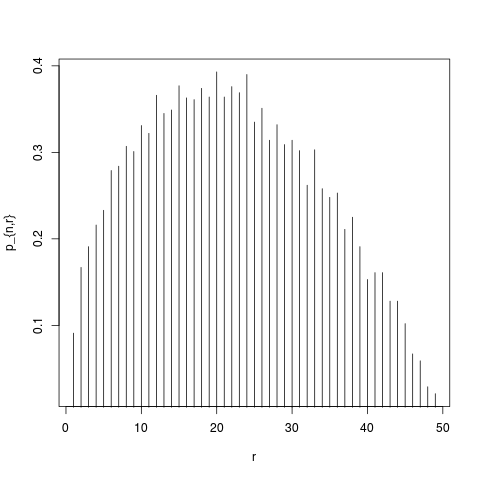
\includegraphics[width=12cm,height=9cm,keepaspectratio]{ej3.png}\\


\section*{Ejercicio 4: gráfico comparativo de $r_n$ con $n$}
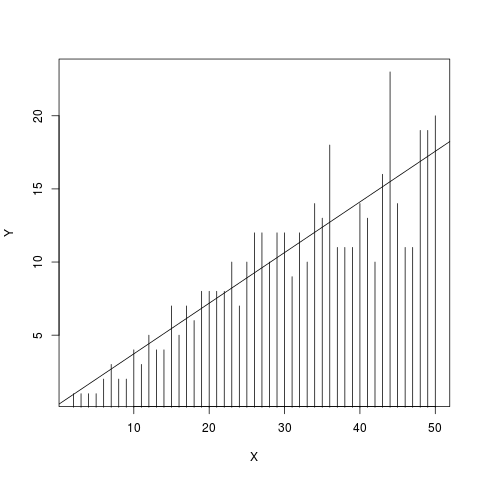
\includegraphics[width=12cm,height=9cm,keepaspectratio]{ej4.png}

Graficamos como $r_n$ el promedio de 10 corridas de la aproximación para tratar de suavizar la función obtenida, obteniendo una aproximación más precisa de cada $r_n$. Se puede notar una dependencia lineal, aunque con algún ruido debido a nuestras aproximaciones.

\section*{Ejercicio 5: mostrar empíricamente que el límite converge a $e$}
La pendiente del mejor ajuste lineal del gráfico $r_n$ vs $n$ , según nuestro script, es 0.3692 . Lo que significa que $n/r_n$ según el ajuste es $1/0.3692 = 2.708$, que vemos que está cerca del valor real de $e =~ 2.718282 $. Simulando para valores más grandes de $n$, obtenemos lo siguiente:
\\
\begin{verbatim}
[1] Ej 5
[1] "n = 50 ; avg_r_n = 18 ; n/r_n = 2.77777777777778"
[1] "n = 100 ; avg_r_n = 37.7 ; n/r_n = 2.6525198938992"
[1] "n = 150 ; avg_r_n = 57.1 ; n/r_n = 2.62697022767075"
[1] "n = 300 ; avg_r_n = 101.4 ; n/r_n = 2.9585798816568"
\end{verbatim}

Esta salida es corriendo a nuestro script pasándole como semilla el número $1$.
\\

También graficamos lo obtenido pero las estimaciones son ruidosas y posiblemente la velocidad de convergencia es lenta. Para los valores de $n/r_n$ que pudimos computar no se ve una clara convergencia, aunque sí se ve que los valores son todos cercanos a $e$ (línea horizontal). Suponemos el ajuste lineal da mucho mejor porque los errores entre las mediciones individuales se compensan, y termina ajustando a una función muy similar a una lineal de slope $e$.

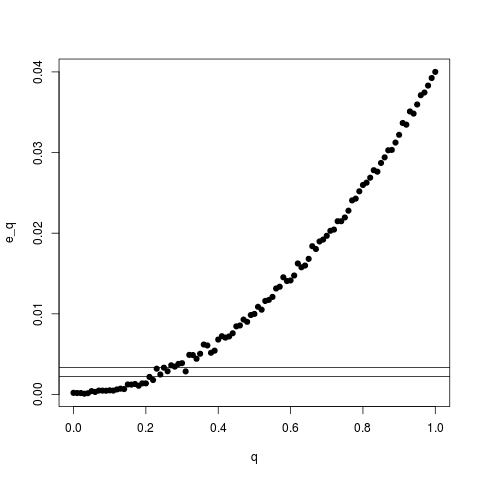
\includegraphics[width=12cm,height=9cm,keepaspectratio]{ej5.png}

\section*{Ejercicio 7: demostración analítica del límite anterior}

Calcularemos la probabilidad $p_{n,r}$. Para ello, fijaremos $n$ y $r$ y llamaremos $a_i$ al valor que tiene le candidate $i$ dada una permutación de las $n!$ posibles.

Llamemos $C_i$ a la proposición "\textit{le mejor candidate está en la posición $i$}" y particionemos el espacio por $C_i$ con $i=1,\ldots,n$ pues son eventos disjuntos tales que la unión de ellos forma el conjunto completo de las posibles situaciones. Tenemos que:\\

$$P(\text{elegir al mejor candidato}) = \sum_{i=1}^{n}P(\text{elegir al mejor candidato} \ | \ C_i)*P(C_i)$$

Sabemos que $P(C_i) = \frac{1}{n}$ pues las $n!$ permutaciones son equiprobables. Luego, solo falta calcular $P(\text{elegir al mejor candidato} \ | \ C_i)$ para cada $i$.\\

Si $i \leq r$, se tiene que $P(\text{elegir al mejor candidato} \ | \ C_i) = 0$. Esto es porque le mejor candidate está en una posición que será descartada automáticamente. \\

A continuación calcularemos $P(\text{elegir a le mejor candidate} \ | \ C_i)$ con $i = r+1, r+2 \ \text{y} \ r+3$ para dar intuición del cálculo general.
\begin{itemize}
    \item Caso $i = r+1$. Como le mejor candidate está en la posición $r+1$, no importa a quiénes descartemos en las primeras $r$ posiciones elegiremos el/la $r+1$-ésimx candidatx, que será mayor a todxs ellxs. Por lo tanto, $P(\text{elegir a le mejor candidate} \ | \ C_{r+1}) = 1$.
    \item Caso $i = r+1$. Para calcularlo tenemos que contar entre todas las permutaciones posibles donde $a_{r+2} = n$, en cuántas de ellas $a_{r+1} < \displaystyle\max_{1 \leq i \leq r} a_i$ (esta condición es la necesaria para no elegir $a_{r+1}$ y entonces elegir pasar al siguiente, que es el/la mejor de todxs). \\

Por simplicidad en el análisis calcularemos cuál es la probabilidad de \textbf{no} elegir al mejor candidatx. Notemos que la probabilidad de que suceda esto es igual a la probabilidad de que el mejor de los primeros $r+1$ esté en la última posición, sin importar cuáles son estos valores. Esa probabilidad es $\dfrac{1}{r+1}$. Por lo tanto, la probabilidad de elegir al mejor dado que $a_{r+2} = n$ es $1 - \dfrac{1}{r+1} = \dfrac{r}{r+1}$
    \item Caso $i = r+3$. Análogamente al caso anterior, calcularemos la probabilidad de \textbf{no} elegir al mejor candidato. Es decir, la probabilidad de que $\displaystyle\argmax_{1 \leq i \leq r+2} a_i \in \{r+1, r+2\}$, ya que si el mejor de ellos está entre los primeros $r$ por definición del procedimiento no elegiremos ni al $r+1$ ni al $r+2$.\\
    Entonces esta probabilidad es $\dfrac{2}{r+2}$. Por lo tanto, $P(\text{elegir a le mejor candidate} \ | \ C_{r+3}) = 1 - \dfrac{2}{r+2} = \dfrac{r}{r+2}$

\end{itemize}

De aquí se deduce fácilmente la fórmula para el caso general. Si $i = r + k$, queremos calcular la probabilidad de que $\displaystyle\argmax_{1 \leq i \leq r+k-1} a_i \in \{r+1, \ldots, r+k-1\}$, que es $\dfrac{k-1}{r+k-1}$.\\

$$P(\text{elegir a le mejor candidate} \ | \ C_{r+k}) = 1 - \dfrac{k-1}{r+k-1} = \dfrac{r}{r+k-1}$$
\\

Entonces finalmente tenemos que:\\
$$P(\text{elegir a le mejor candidate}) = \sum_{i=1}^{n}P(\text{elegir a le mejor candidate} \ | \ C_i) \cdot P(C_i) = \sum_{i=r+1}^{n} \dfrac{r}{i-1} \cdot \dfrac{1}{n} = \dfrac{r}{n} \sum_{i=r}^{n-1} \dfrac{1}{i}$$

Lo último que nos falta es dar una estimación para $\dfrac{r}{n} \displaystyle\sum_{i=r}^{n-1} \dfrac{1}{i}$, que no tiene fórmula cerrada conocida.

\subsection*{Estimación de $\displaystyle\sum_{i=r}^{n-1} \dfrac{1}{i}$}
No hay una fórmula cerrada para $\displaystyle\sum_{i=r}^{n-1} \dfrac{1}{i}$, pero lo que podemos hacer es aproximarlo con la integral $$\int_{r}^{n} \dfrac{1}{x} dx$$

Gráficamente, lo podemos pensar como un gráfico de barras de ancho $1$ y altura $\dfrac{1}{i}$, y si bien para valores chicos de $i$ la aproximación no es buena, para valores grandes la función $\dfrac{1}{x}$ se vuelve bastante 'horizontal', teniendo en un ancho de $1$ un cambio de altura chico ($1/x$ se parece a $1/(x+1)$). Entonces podemos pensar en aproximar a esa sumatoria como el área debajo de la curva $1/x$ con $x$ entre $r$ y $n$. Acá el límite superior es $n$ porque como en la sumatoria queríamos sumar desde $r$ hasta $n-1$, si asignamos un ancho de medida $1$, el valor de $1/r$ lo consideramos desde $x = r$ hasta $x = r+1$, y así sucesivamente.\\

Entonces, integrando, obtenemos $$\int_{r}^{n} \dfrac{1}{x} dx = \ln(n) - \ln(r) = \ln\Big(\dfrac{n}{r}\Big)$$. \\

Finalmente, retomando la ecuación obtenida anteriorment podemos aproximar $p_{n,r}$ por $\Bar{p}_{n,r}= \dfrac{r}{n} \ln\Big(\dfrac{n}{r}\Big)$.\\

Si pensamos en el gráfico de esa función como función de $r$ (que gracias a nuestra aproximación es continua), podemos ver que cuando $r$ tiende a $0$ la función se acerca a $0$ (como vimos en el punto $1$, que si $r$ es chico la probabilidad también), y si $r = n$ la función vuelve a valer $0$ (que tiene sentido ya que significa descartar a todes les candidates. Entonces, como es continua, debe haber por lo menos un valor intermedio en donde la función tome su valor máximo. Si pensamos en el problema esto tiene sentido ya que debe haber un equilibrio entre la cantidad de información que queremos adquirir (gente descartada) y el momento a partir del cual empezamos a buscar al mejor.
Derivando nuestra expresión en función de $r$:\\

$$\Bar{p}_{n,r}' = \dfrac{1}{n} \cdot \Big[\ln\Big(\dfrac{n}{r}\Big) - 1\Big]$$.
\\

Finalmente igualando la derivada a $0$ para encontrar $\Bar{r}_n$ obtenemos $\ln\Big(\dfrac{n}{\Bar{r}_n}\Big) = 1 \Rightarrow \dfrac{n}{\Bar{r}_n} = e \Rightarrow \Bar{r}_n = \dfrac{n}{e}$.

Ahora, esto salió de usar la aproximación de la función $1/x$ para la sumatoria, que cuando $n$ tiende a infinito es cada vez más acertada (ya que lógicamente $r_n$ crece), obteniendo el límite deseado.\\


Esto también nos permite calcular la probabilidad conjeturada en el ejercicio 5 ahora que sabemos que $r_n$ tiende a $\dfrac{n}{e}$:

$$\Bar{p}_{n,r_n} = \dfrac{r_n}{n} \ln\Big(\dfrac{n}{r_n}\Big)$$

$$\lim_{n \rightarrow \infty} p_{n,r_n} = \dfrac{r_n}{n} \ln\Big(\dfrac{n}{r_n}\Big) = \dfrac{n/e}{n} \ln\Big(\dfrac{n}{n/e}\Big) = \dfrac{1}{e}$$

\section*{Ejercicio 8: ¡hemos sido engañados!}

La estrategia presentada en el enunciado del TP es óptima, como muestra por ejemplo Bruss 2000 (\url{https://projecteuclid.org/download/pdf_1/euclid.aop/1019160340}).

\end{document}
